\section{Results}


\subsection{Outflow Identification}

\begin{table}[h!]
	\caption{Protostars with observed outflows.}
	\label{protostars}
	\begin{center}
		\begin{tabular}{c|c|c|c|c}
			\toprule
			& \multicolumn{2}{c|}{coordinates} & $\mathbf{L_{bol}}$ & $\mathbf{T_{bol}}$\\
			\textbf{Name} & \textbf{RA} & \textbf{Dec} & $\mathbf{L_{\odot}}$ & $\mathbf{K}$\\
			\midrule
			\centering
			FIR2 & 05:35:24.3 & -05:08:33.3 & 5.68 & 100.6\\
			FIR3 & 05:35:27.5 & -05:09:32.5 & 360.86 & 71.5\\
			FIR6b & 05:35:23.4 & -05:12:03.2 & 21.93 & 54.1\\
			MMS2 & 05:35:18.3 & -05:00:34.8 & 20.11 & 186.3\\
			MMS5 & 05:35:22.4 & -05:01:14.1 & 15.81 & 42.4\\
			MMS9 & 05:35:26.0 & -05:05:42.4 & 8.91 & 38.1\\
			\midrule
		\end{tabular}
	\end{center}
\end{table}
Table \ref{protostars} shows the protostars with bipolar outflows observed. 

\subsubsection{$^{12}$CO J = 2 - 1 Observations}

\begin{figure}[h!]
	\begin{center}
		\begin{tabular}{cc}
			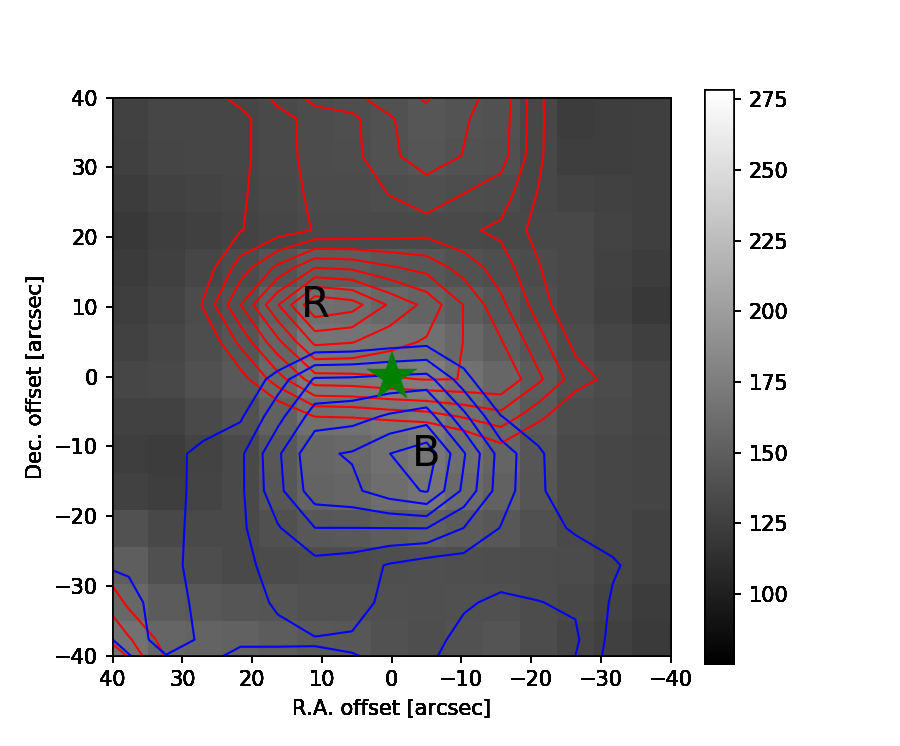
\includegraphics[width=7cm]{Orion_12CO2-1_FIR2_rbcontour_400_modified.png} &   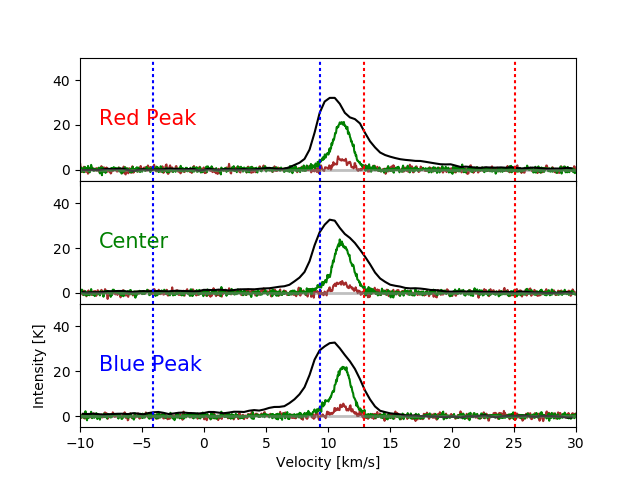
\includegraphics[width=7cm]{Orion_12CO2-1_FIR2_line_profile_400.png} \\
		\end{tabular}
		\label{FIR221}
		\caption{The contour map(left) and the line profile(right) of FIR2. }
	\end{center}
\end{figure}

\begin{figure}[h!]
	\begin{center}
		\begin{tabular}{cc}
			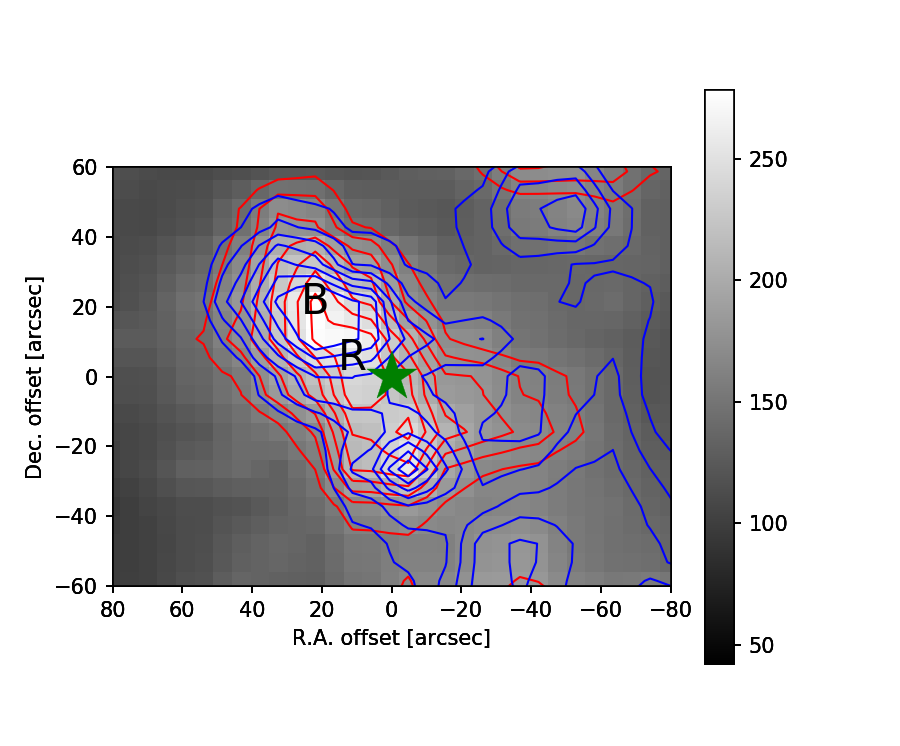
\includegraphics[width=7cm]{Orion_12CO2-1_FIR3_rbcontour_400_modified.png} &   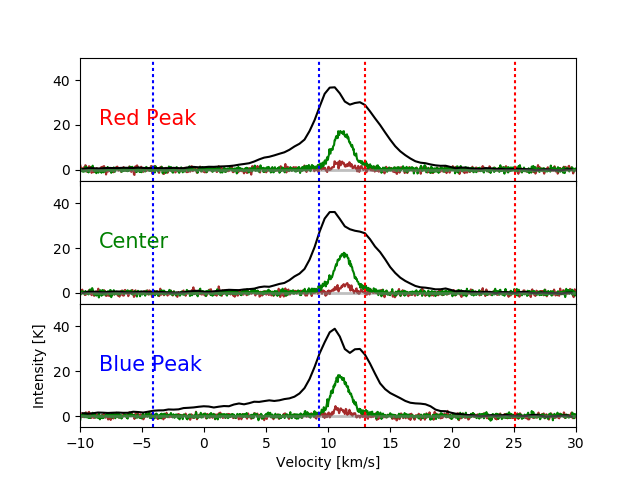
\includegraphics[width=7cm]{Orion_12CO2-1_FIR3_line_profile_400.png}\\
		\end{tabular}
		\label{FIR321}
		\caption{The contour map and the line profile of FIR3. }
	\end{center}
\end{figure}

\begin{figure}[h!]
	\begin{center}
		\begin{tabular}{cc}
			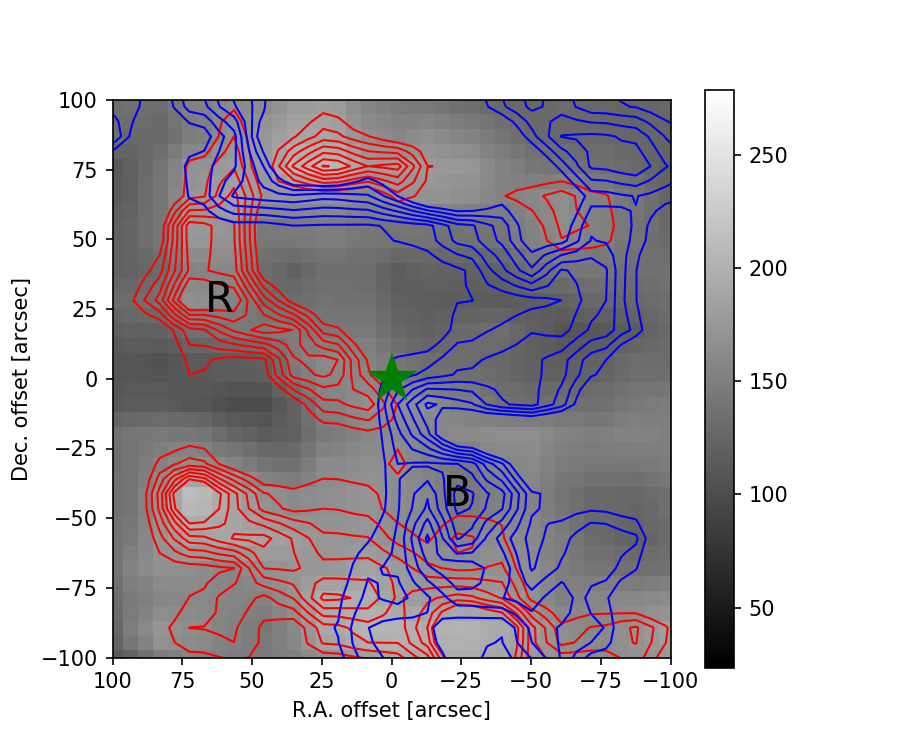
\includegraphics[width=7cm]{Orion_12CO2-1_FIR6b_rbcontour_400_modified.png} &   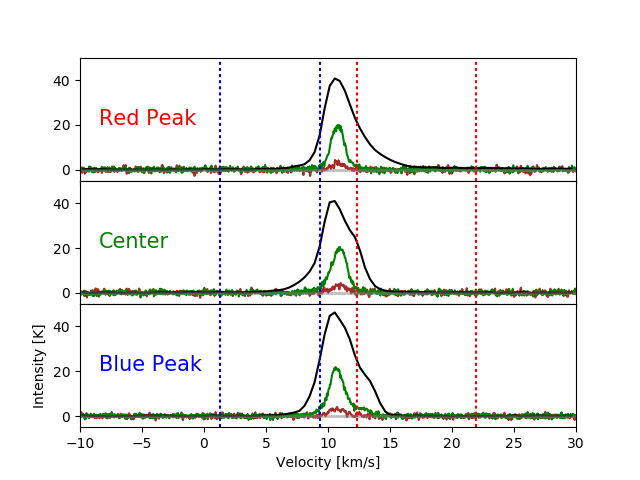
\includegraphics[width=7cm]{Orion_12CO2-1_FIR6b_line_profile_400.png}\\
		\end{tabular}
		\label{FIR6b21}
		\caption{The contour map and the line profile of FIR6b. }
	\end{center}
\end{figure}

\begin{figure}[h!]
	\begin{center}
		\begin{tabular}{cc}
			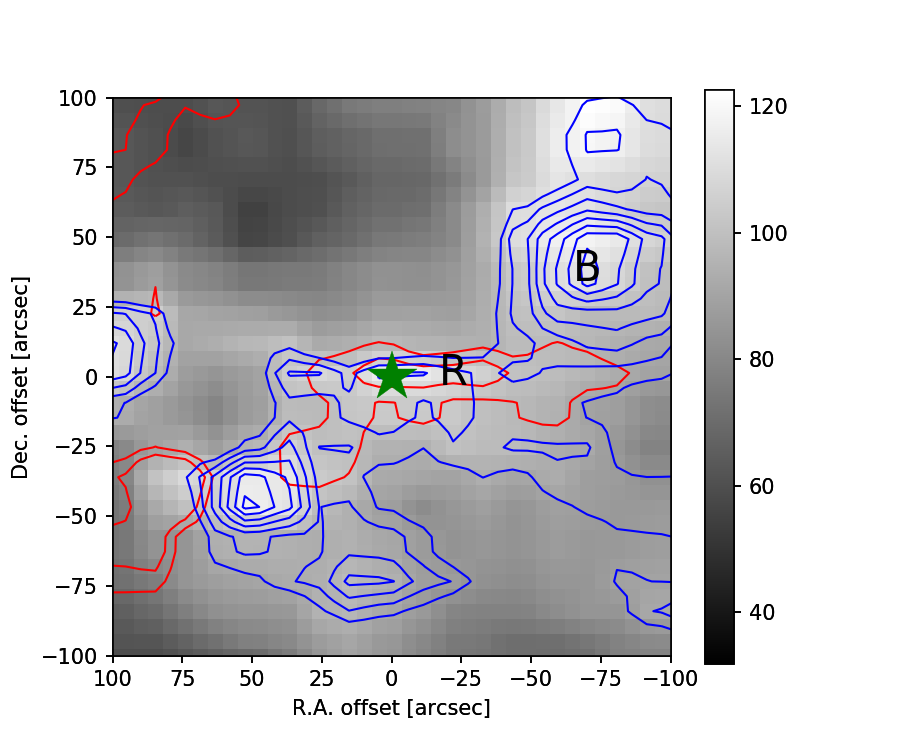
\includegraphics[width=7cm]{Orion_12CO2-1_MMS2_rbcontour_400_modified.png} &   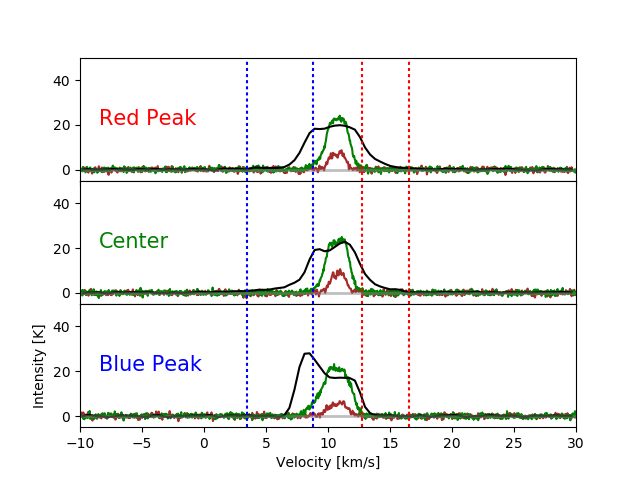
\includegraphics[width=7cm]{Orion_12CO2-1_MMS2_line_profile_400.png} \\
		\end{tabular}
		\label{MMS221}
		\caption{The contour map and the line profile of MMS2. }
	\end{center}
\end{figure}

\begin{figure}[h!]
	\begin{center}
		\begin{tabular}{cc}
			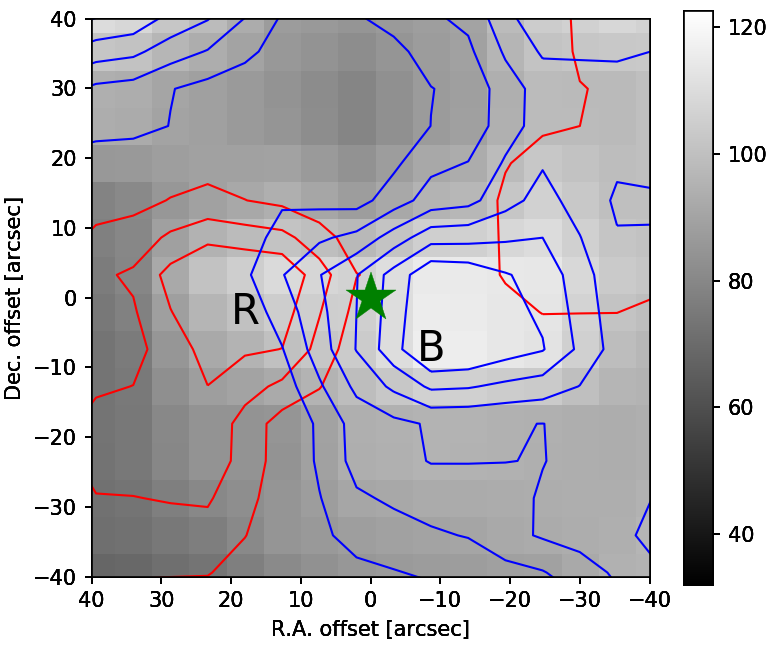
\includegraphics[width=7cm]{Orion_12CO2-1_MMS5_rbcontour_400_modified.png} &   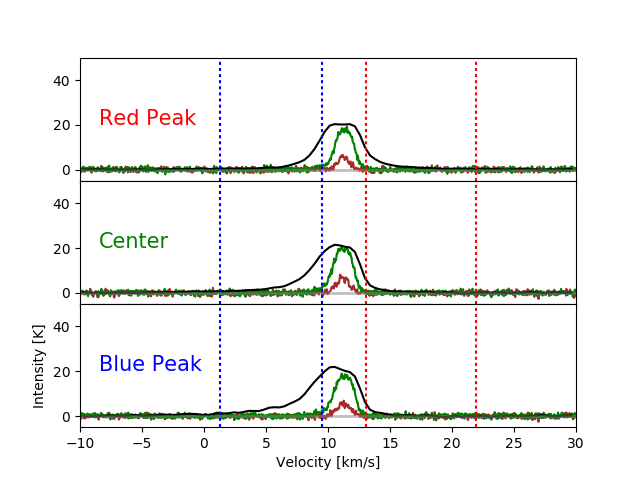
\includegraphics[width=7cm]{Orion_12CO2-1_MMS5_line_profile_400.png} \\
		\end{tabular}
		\label{MMS521}
		\caption{The contour map and the line profile of MMS5. }
	\end{center}
\end{figure}
\clearpage
\newpage
\begin{figure}[h!]
	\begin{center}
		\begin{tabular}{cc}
			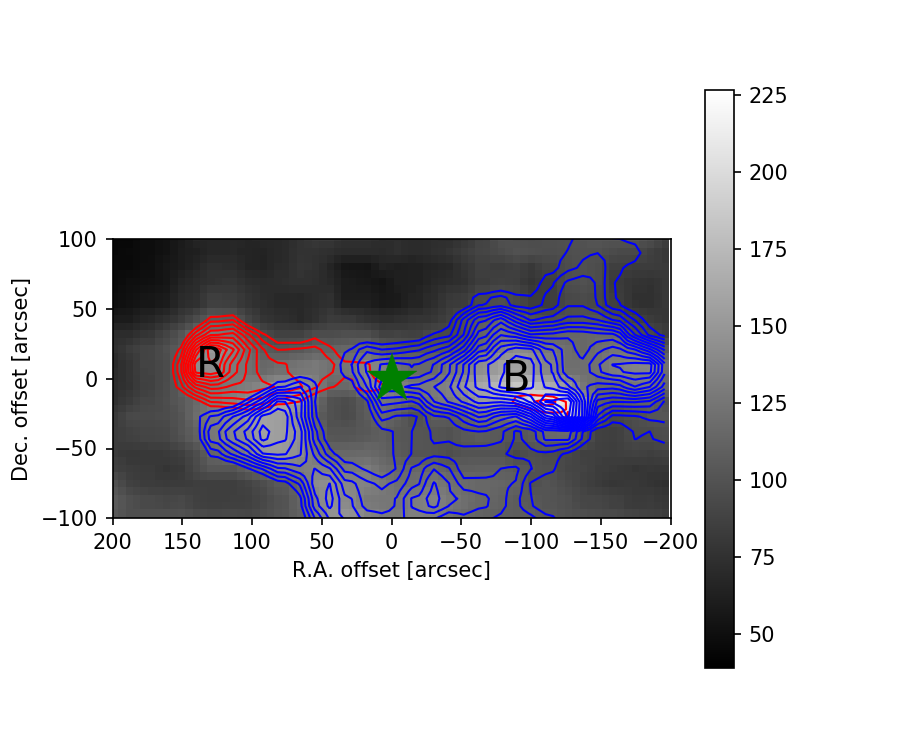
\includegraphics[width=7cm]{Orion_12CO2-1_MMS9_rbcontour_400_modified.png} &   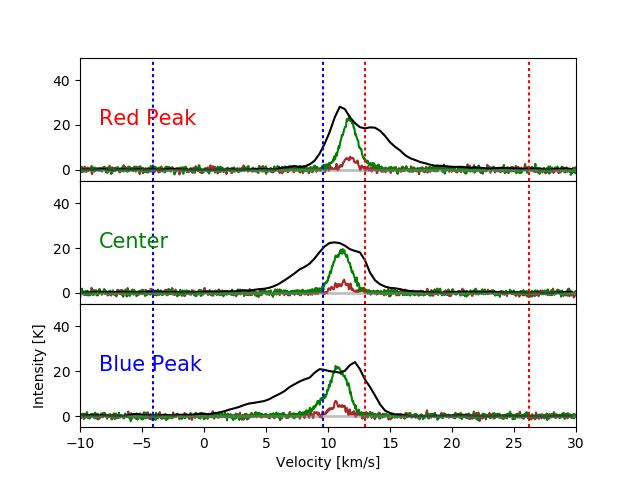
\includegraphics[width=7cm]{Orion_12CO2-1_MMS9_line_profile_400.png} \\
		\end{tabular}
		\label{MMS921}
		\caption{The contour map and the line profile of MMS9. }
	\end{center}
\end{figure}


\noindent\textbf{FIR2} - There is a strong bipolar outflow elongated along the N-S direction as shown in Figure \ref{FIR221}. The size is about 30 arcsec, which is smaller than other outflows detected. Red and blue contour intervals are $10\sigma$ starting from $60\sigma$, and $10\sigma$ starting from $100\sigma$, respectively.\\
\textbf{FIR3} - A strong bipolar outflow can be seen along NE-SW direction, with red and blue lobes overlapped with each other as shown in Figure \ref{FIR321}. This tells us that the outflow axis is almost parallel to the line of sight. Red and blue contour intervals are $20\sigma$ starting from $40\sigma$, and $20\sigma$ starting from $60\sigma$, respectively. \\
\textbf{FIR6b} - The contour is not so clear because of other IR sources nearby as shown in Figure \ref{FIR6b21}. The outflow is along the NW-SE direction. Red and blue contour intervals are $10\sigma$ starting from $45\sigma$, and $10\sigma$ starting from $110\sigma$, respectively.\\
\textbf{MMS2} - The contour is in a tricky situation, because both red and blue lobes are in the east side of the protostar as shown in Figure \ref{MMS221}. The outflow structure on the SW side is the outflow from another protostar, MMS5. It is possible that the outflow structure changed shape because of the turbulence from other protostars. Red and blue contour intervals are $10\sigma$ starting from $30\sigma$, and $10\sigma$ starting from $60\sigma$, respectively.\\
\textbf{MMS5} - There is an outflow structure along the E-W direction as shown in Figure \ref{MMS521}. This outflow is much smaller than other bipolar outflows. Red and blue contour intervals are $10\sigma$ starting from $20\sigma$, and $10\sigma$ starting from $40\sigma$, respectively.\\
\textbf{MMS9} = There is a strong outflow along the E-W direction as shown in Figure \ref{MMS921}. We can see a smaller red lobe near the center of the blue lobe. Red and blue contour intervals are $10\sigma$ starting from $50\sigma$, and $10\sigma$ starting from $60\sigma$, respectively.\\

\subsubsection{$^{12}$CO J = 1 - 0 Observations}

\begin{figure}[h!]
	\begin{tabular}{ccc}
		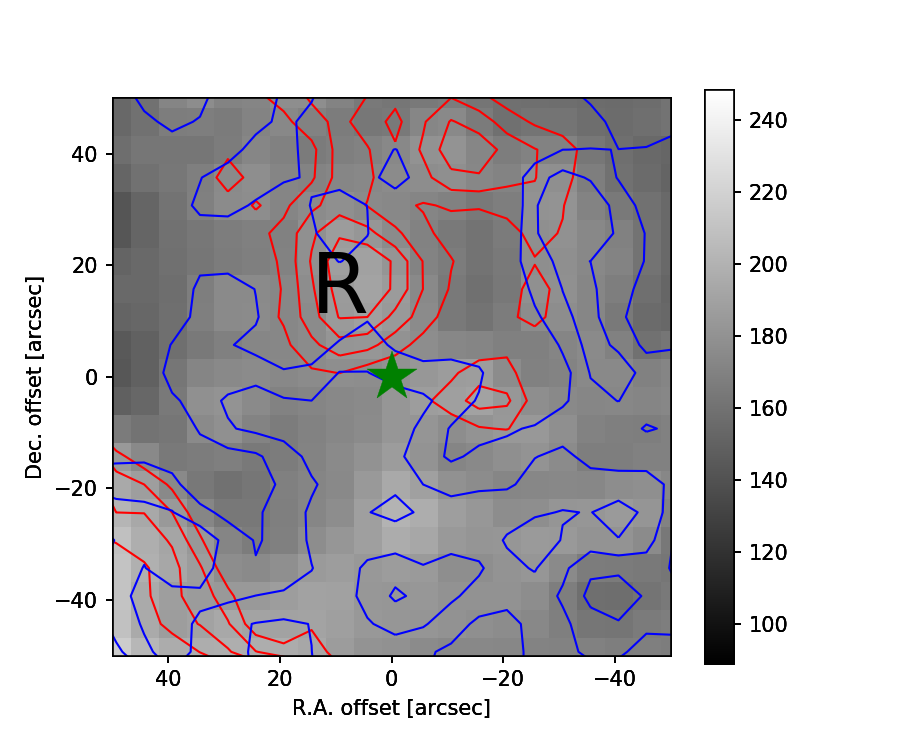
\includegraphics[width = 5cm]{Orion_12CO_NRO_HOPS68_rbcontour_400.png} & 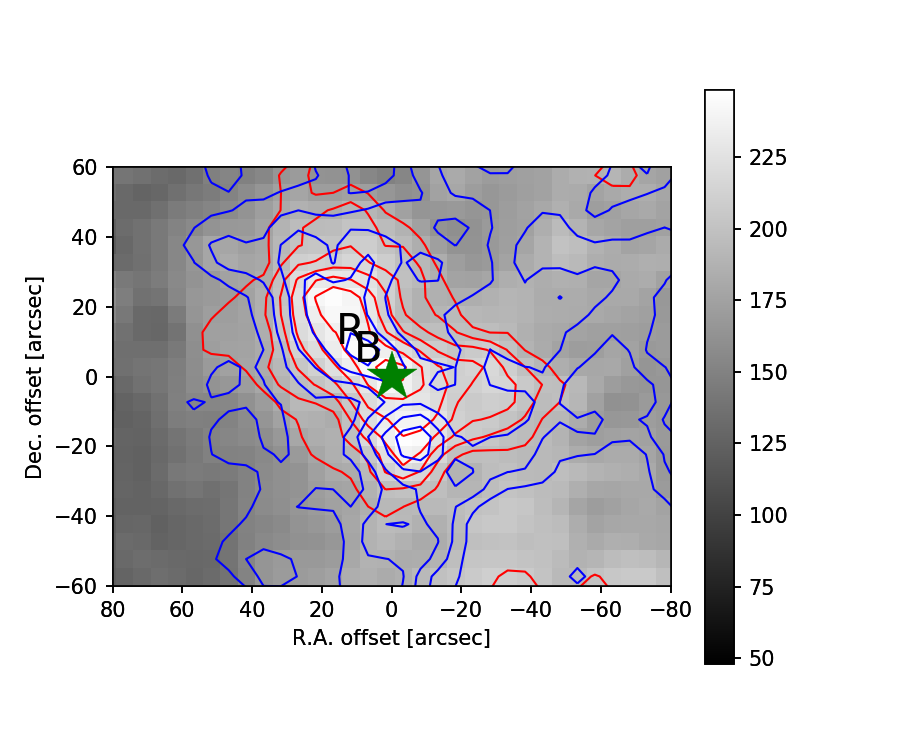
\includegraphics[width = 5cm]{Orion_12CO_NRO_HOPS370_rbcontour_400.png} & 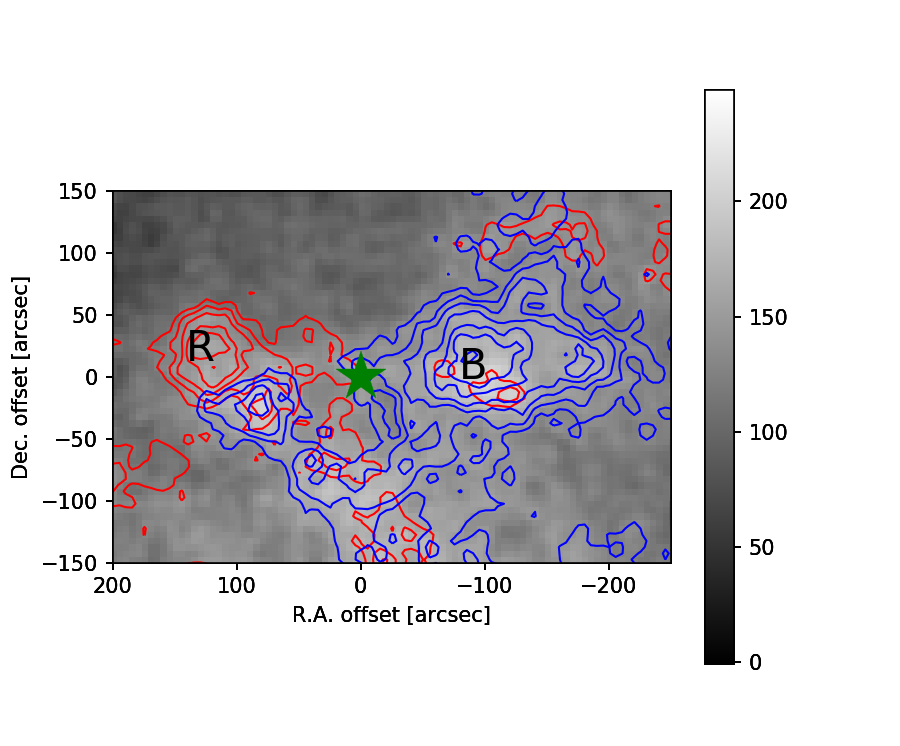
\includegraphics[width = 5cm]{Orion_12CO_NRO_HOPS78_rbcontour_400.png}
		\label{10}
	\end{tabular}
	\caption{The contour map of FIR2(left), FIR3(middle), and MMS9(right). }
\end{figure}
 
 
\noindent \textbf{FIR2} - The red lobe is clear on the NW side of the protostar, but the blue lobe is not that clear as shown in Figure \ref{10}.\\
\textbf{FIR3} - The outflows are in a similar shape with the J = 2 - 1 observations as shown in Figure \ref{10}. The lobe centers are slightly near the protostar.\\
\textbf{MMS9} - The outflows are also in a similar shape with the J = 2 - 1 observations as shown in Figure \ref{10}. We can also see that there is a small red lobe near the center of the blue lobe.\\
\newpage

\subsection{Momentum Flux}


\begin{table}[h]
	\caption{CO outflow parameters.} \label{result}
	\begin{center}
		\begin{tabular}{c|c|c|c||c|c|c}
			\toprule
			\multirow{3}{1cm}{\textbf{Name}} & \multicolumn{3}{c}{J = 2 - 1} & \multicolumn{3}{c}{J = 1 - 0} \\
			& $\mathbf{F_{R}}$ & $\mathbf{F_{B}}$ & $\mathbf{F_{\textrm{\textbf{CO}}}}$ & $\mathbf{F_{R}}$ & $\mathbf{F_{B}}$ & $\mathbf{F_{\textrm{\textbf{CO}}}}$\\
			& \multicolumn{6}{c}{($M_{\odot} \, \textrm{km s}^{-1} \textrm{yr}^{-1}$)}\\
			\midrule
			FIR2 & 1.14E-05 & 3.28E-05 & 4.42E-05 & 4.78E-06 & - & 4.78E-06\\
			FIR3 & 4.77E-04 & 7.43E-04 & 1.22E-03 & 1.86E-04 & 3.02E-04 & 4.88E-04\\
			FIR6b & 1.13E-05 & 1.18E-05 & 2.31E-05 & - & - & -\\
			MMS2 & 1.14E-05 & 4.50E-05 & 5.64E-05 & - & - & -\\
			MMS5 & 5.80E-06 & 1.55E-05 & 2.13E-05 & - & - & -\\
			MMS9 & 3.67E-06 & 1.09E-05 & 1.46E-05 & 1.45E-06 & 6.02E-06 & 7.47E-06\\
			\toprule
		\end{tabular}
	\end{center}
\end{table}


Table \noindent\ref{result} shows the parameters of the outflows detected. $F_R$ and $F_B$ stands for the outflow forces for the red lobe and the blue lobe respectively. $F_{\textrm{CO}}$ is calculated by adding the two forces, which shows the momentum flux of the protostar. We can see that more outflows were detected by using J = 2 - 1 data, and the momentum flux is 2-3 times higher.\\

\clearpage
\newpage
\subsection{Momentum flux vs. Bolometric luminosity}


\begin{figure}[h!]
	\centering
	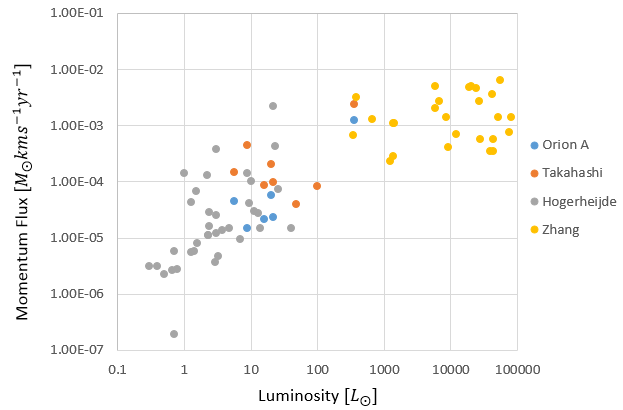
\includegraphics[width=\textwidth]{Luminosity}
	\label{lum}
	\caption{Momentum flux difference by emission line energy.}
\end{figure}


Figure \ref{lum} shows the relation between the bolometric luminosity and the momentum flux of the outflows from previous studies \cite{takahashi2008millimeter, van2013outflow, hogerheijde1998envelope, nakamura2012evidence, aso2000dense, zhang2005search}. \\ Since the momentum flux of the same protostar is known to vary somewhat depending on the calculation methods\cite{van2013outflow}, the relation between the bolometric luminosity and the momentum flux is difficult to express with the excat formula and only the degree of tendency can be analyzed.
The bolometric luminosity was observed by the Spitzer and Herschel telescopes. Orion A Cloud is a region where stars with medium mass are formed. The fact that the momentum flux of the outflow is proportional to the bolometric luminosity could be checked.

\newpage

\subsection{Momentum flux by emission line energy level}

\begin{figure}[h!]
	\centering
	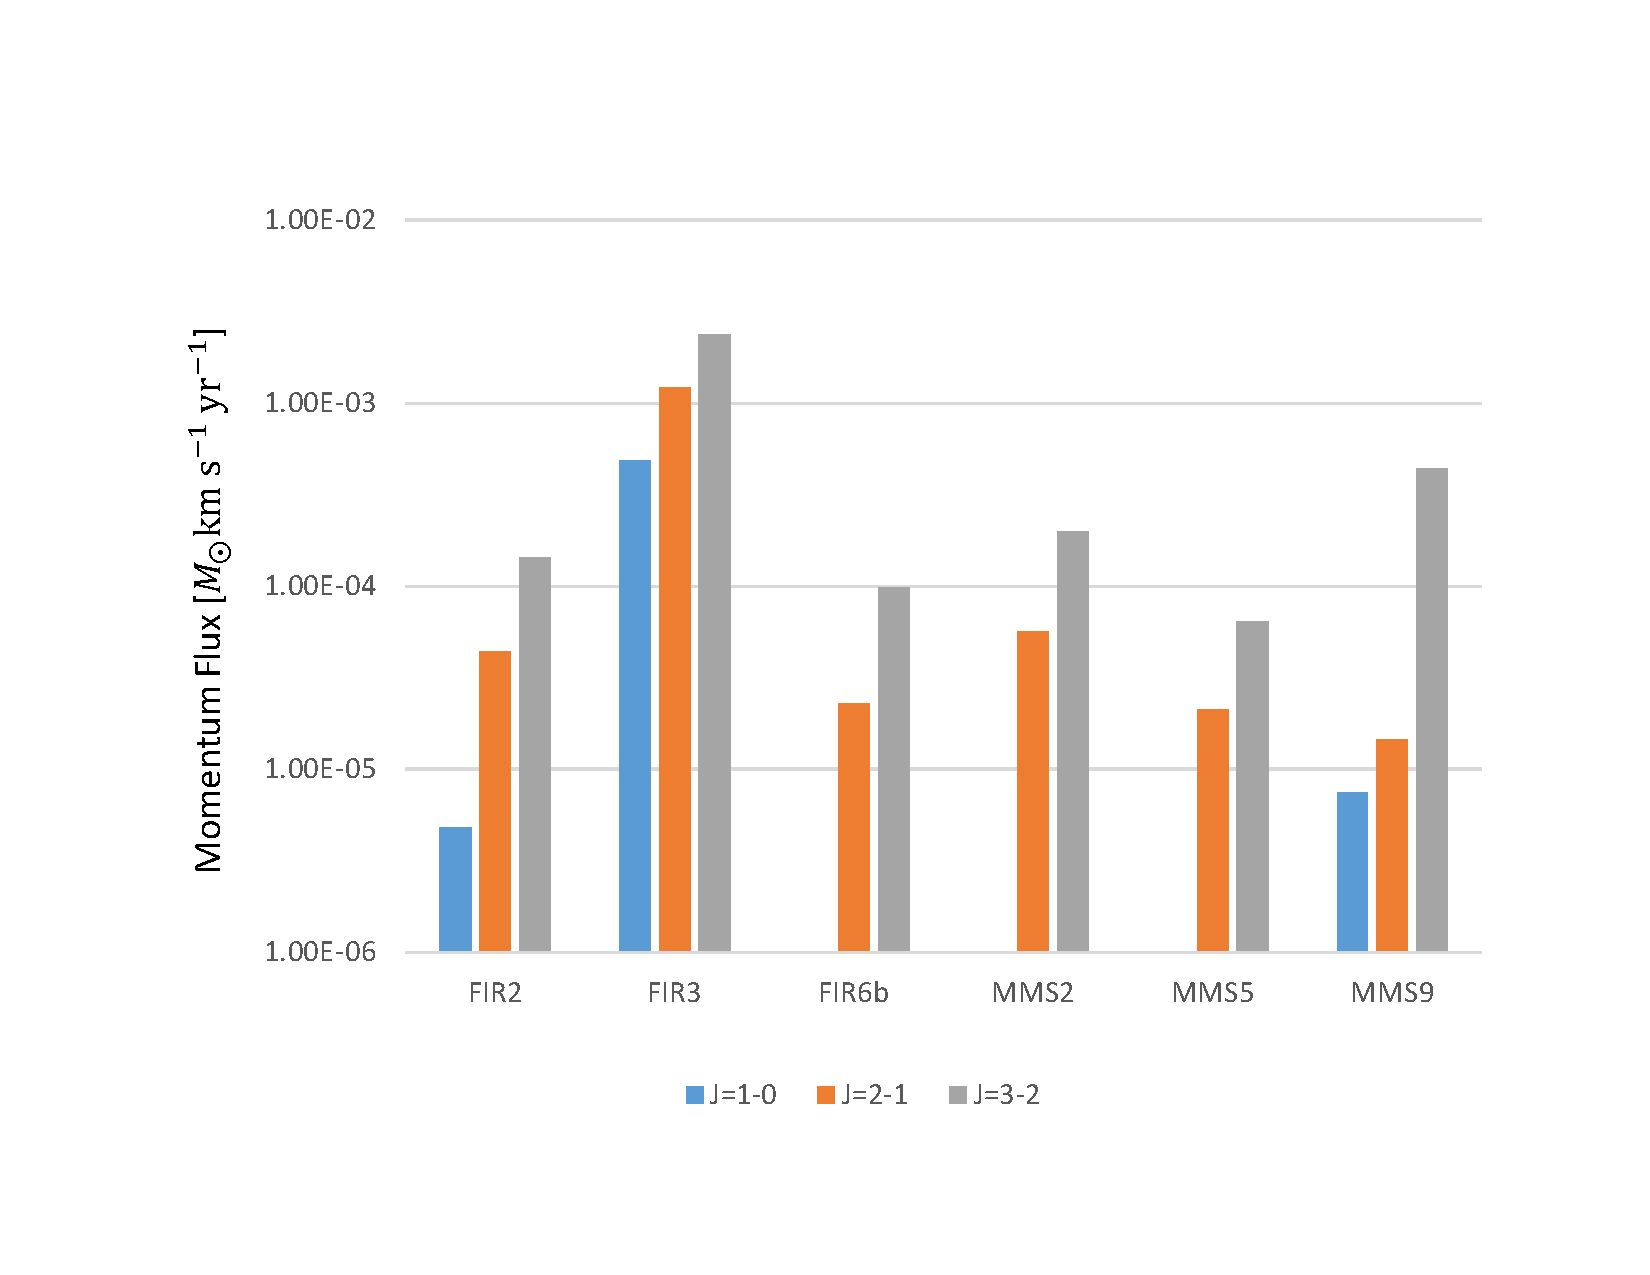
\includegraphics[width=\textwidth]{outflow_J}
	\ref{J}
	\caption{Momentum flux difference by emission line energy.}
\end{figure}

Figure \ref{J} compares momentum flux calculated by three different emission lines of the same protostar. The $^{12}$CO J = 3 - 2 observation was made by Takahashi et al \cite{takahashi2008millimeter}. We can see that it is possible to detect more outflows by using a higher energy emission line of $^{12}$CO. Using data with smaller beamwidth also enhances detecting outflows. The reason that higher energy lines can detect more outflows can be explained as the following. The excitation temperature is higher for emission lines with higher energy. Outflows drag out matter from the protostar's envelope, which has higher temperature than its surroundings. Lines with higher energy are emitted, which has an effect that makes column density higher than usual.